\chapter{Basis Splines}\label{B-splines}
A basis spline, or B-spline, of order $k$ is a piecewise polynomial function of degree $(k-1)$ defined on a collection of points, $t_i$, called \textit{knot points}. The array formed by these knot points are referred to as \textit{knot sequence}, or knot vector, where $t_i\leq t_{i+1}$. B-splines of order $k$ can be defined recursively by the Cox-de Boor formula. With a given knot sequence, the B-splines of order $k=1$ are defined as

\begin{equation}
B_{i,k=1}(x) \doteq
\begin{cases}
1, \quad \text{if} \quad & t_i \leq x < t_{i+1}\\
0,& \text{otherwise} 
\end{cases}
\end{equation}
and if $k>1$

\begin{equation}
B_{i,k}(x) \doteq \frac{x-t_i}{t_{i+k-1}-t_i}B_{i,k-1}(x) + \frac{t_{i+k}-x}{t_{i+k}-t_{i+1}}B_{i+1,k-1}(x).
\end{equation}
The B-splines are local in the sense that they will be non-zero only in a limited region of space. If the numbering is such that the first knot point is $t_1$ and the first  B-spline is $B_{1,k}$, then the B-spline $B_{i,k}$ is non-zero within the region $t_i \leq x \leq t_{i+k}$. On a given knot sequence $(t_1,\ldots , t_P)$ the B-splines form a complete set

\begin{equation}
\sum_{i=1}^{P} B_{i,k}(x) = 1.
\end{equation}
By placing $(k-1)$ additional points, called \text{ghost points}, at the end-points, the B-splines will be confined within the region $t_1 \leq x \leq t_P$. This means that $P$ knot points correspond to $N=P-2(k-1)$ physical points. B-splines of orders $k=1-4$ are shown in \cref{fig:B-spline}. The first derivative of a B-spline of order $k$ is given by

\begin{equation}
\frac{\partial}{\partial x}B_{i,k}(x) = (k-1)\bigg(\frac{B_{i,k-1}(x)}{t_{i+k-1}-t_i} + \frac{B_{i+1,k-1}(x)}{t_{i+k}-t_{i+1}}\bigg),
\end{equation}
and the second derivative by

\begin{align}
\frac{\partial^2}{\partial x^2}B_{i,k}(x) &= \frac{(k-1)(k-2)B_{i,k-2}(x)}{(t_{i+k-1}-t_i)(t_{i+k-2}-t_i)} - \frac{(k-1)(k-2)B_{i+1,k-2}(x)}{(t_{i+k-1}-t_i)(t_{i+k-1}-t_{i+1})}\nonumber\\
&- \frac{(k-1)(k-2)B_{i+1,k-2}(x)}{(t_{i+k}-t_{i+1})(t_{i+k-1}-t_{i+1})} +  \frac{(k-1)(k-2)B_{i+2,k-2}(x)}{(t_{i+k}-t_{i+1})(t_{i+k}-t_{i+2})}.
\end{align}

The approach of placing the ghost points in the end-points is common because at the first physical point only the first B-spline will be non-zero and only the first two B-splines will have non-zero derivatives. Likewise, at the last physical point only the last B-spline will be non-zero and only the two last B-splines will have non-zero derivatives. Consequently, this choice favours implementation of boundary conditions which require the function or its derivative to be zero at the boundary.

\begin{figure*}[htbp!]
	\centering
	\begin{adjustwidth}{-1cm}{-1cm}
	\begin{subfigure}{0.6\textwidth}
	\centering
	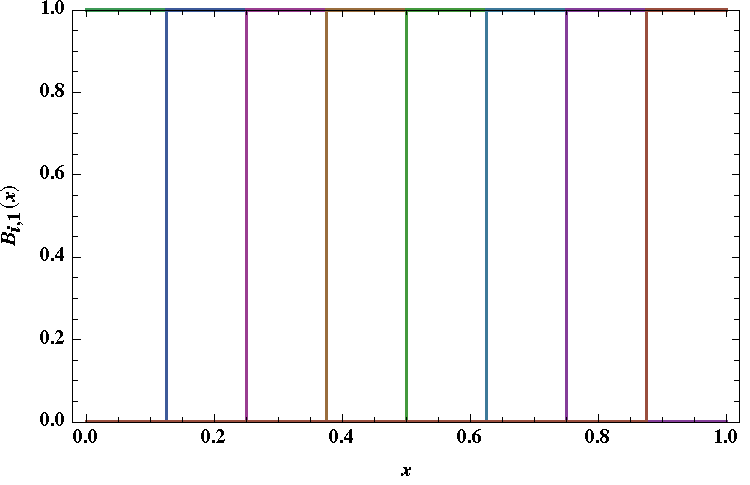
\includegraphics[width=\linewidth]{Bsp1.pdf}
	\caption{$k=1$}
\end{subfigure}%
\begin{subfigure}{0.6\textwidth}
	\centering
	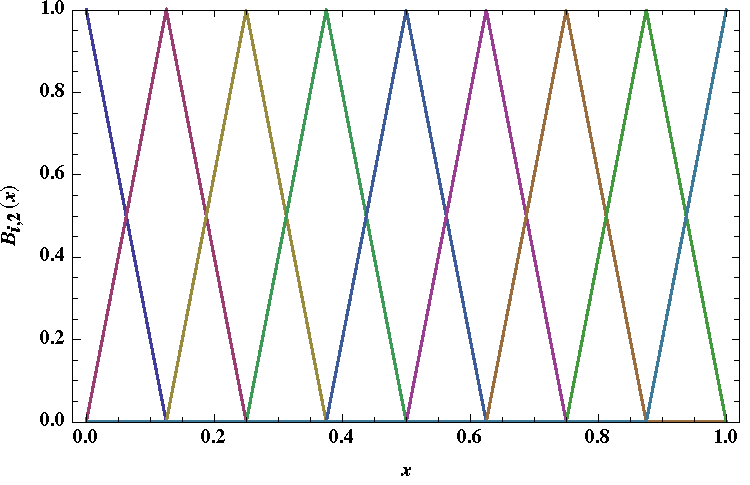
\includegraphics[width=\linewidth]{Bsp2.pdf}
	\caption{$k=2$}
\end{subfigure}%

\begin{subfigure}{0.6\textwidth}
	\centering
	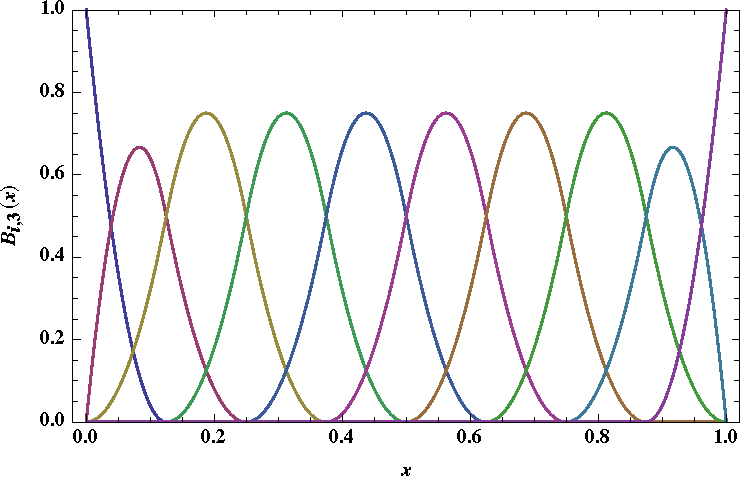
\includegraphics[width=\linewidth]{Bsp3.pdf}
	\caption{$k=3$}
\end{subfigure}%
\begin{subfigure}{0.6\textwidth}
	\centering
	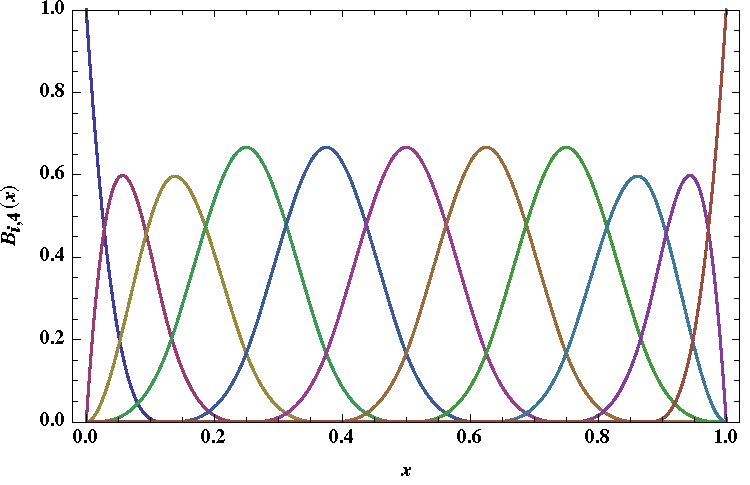
\includegraphics[width=\linewidth]{Bsp4.pdf}
	\caption{$k=4$}
\end{subfigure}%
	\end{adjustwidth}
	\caption{The subfigures above show the B-splines $B_{i,k}(x)$ of different orders $k$ on a one dimensional mesh.}\label{fig:B-spline}
\end{figure*}
